\documentclass{article}

\usepackage{physics} % Handy shortcuts like \pdv, \dd and much more
\usepackage{geometry} % smaller margins, can be adjusted if given arguments
\usepackage{siunitx} % the \si environment for units
\usepackage{mathtools} % The dcases environment, prettier than just cases
\usepackage{tikz} % For drawing picures
\usepackage{wrapfig} % Wrapping text around figures
\usepackage{enumitem} % Getting alphabetical enumerate


\title{Exercise 8 - TFY4345 Classical Mechanics}
\date{2020}

\begin{document}
    \maketitle
    \section{Principal moments of inertia of a triangular slab}
        \begin{wrapfigure}{2}{0.4\textwidth}
            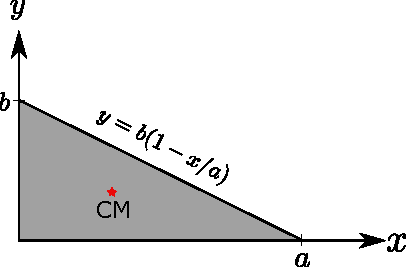
\includegraphics[width=0.4\textwidth]{figures/exercise_1_triangle.pdf}
        \end{wrapfigure}
        (Exam Aug. 2019) 
        \\ \\
        (a) Compute the center-of-mass (CM) for the planar triangle in the figure, assuming it to be of uniform two-dimensional mass density $\rho$.
        \\ \\
        (b) Compute the inertia tensor \emph{with respect to the origin} for the same triangle.
        \\ \\
        (c) (Optional) If the origin is shifted to the CM, the inertia tensor becomes (this can be show by using the Steiner's parallel axis theorem)
        \begin{equation*}
            I_{CM} = 
            \begin{pmatrix*}
                I_{11} & I_{12} & 0 \\
                I_{21} & I_{22} & 0 \\
                0 & 0 & I_{33} \\
            \end{pmatrix*}
             =\frac{M}{18} 
            \begin{pmatrix*}
                b^2 & \frac{1}{2}ab & 0 \\
                \frac{1}{2}ab & a^2 & 0 \\
                0 & 0 & a^2 + b^2 \\
            \end{pmatrix*}
        \end{equation*}
        where $I_{xy} = I_{yx}$ and $I_{xx} + I_{yy} = I_{zz}$ in the general form show first. Define next
        \begin{equation*}
            A = \frac{1}{2}(I_{xx} + I_{yy}), \quad B = \sqrt{\frac{1}{4}(I_{xx} - I_{yy})^2 + I_{xy}^2}, \quad \vartheta = \tan^{-1}\bigg( \frac{2I_{xy}}{I_{xx} - I_{yy}}\bigg).
        \end{equation*}
        Derive the principal moments of inertia and the principal axes by using the general form of the inertia tensor, and these new variables. [Hint] The last equations comprises a relationship that can be described by a right triangle.
    \section{Precession of a frisbee}
        (Exam Aug. 2016) \\ \\
        \begin{figure}
            \centering
            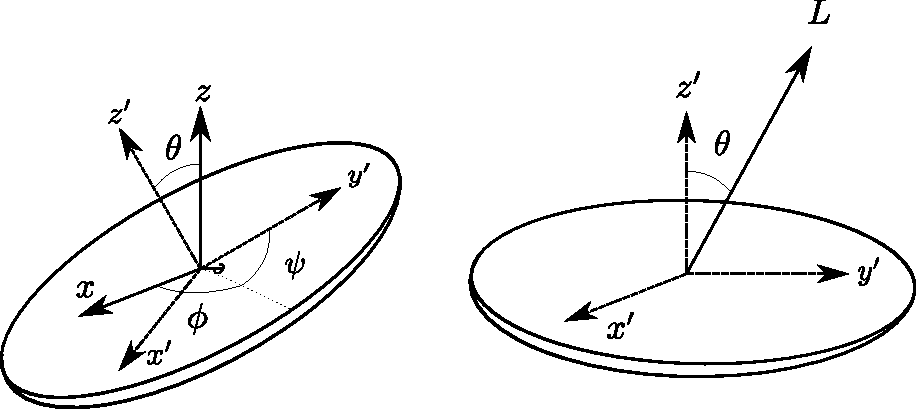
\includegraphics[width=0.8\textwidth]{figures/exercise_2_frisbee.pdf}
        \end{figure}
        Consider an axial-symmetric body with the principal moments of inertia $I_1 = I_2 \neq I_3$, rotating with angular momentum $\mathbf{L} = L \mathbf{e}_z$ in the laboratory frame. (The unmarked coordinate system.)
        \\ \\
        (a) Derive the equations of motion for the body, using the Euler equations and the angles $\theta, \psi$ and $\phi$. Find the components of $\boldsymbol{\omega}$ in the body system. (See lecture notes, we derived this already!)
        \\ \\
        (b) Find the expression for the Euler angles $\dot \theta, \dot \psi, \dot \phi$ as a function of $I_i, L, \theta$.
        \\ \\
        (c) Assume $I_3 = 2I_1$. The precession (wobble) of the frisbee is given by $\dot \phi$. Show that the precession is twice as fast as the rotation frequency of the frisbee, assuming that $\theta$ is small (i.e. that $\cos(\theta) \approx 1$).

    \section{Precession of a heavy spinning top}
        (Based on example p. 208-223 in Goldstein 3rd. ed., p. 70-74 in the compendium)\\
        In the example we define the shifted energy as 
        \begin{equation*}
            E' = \frac{1}{2}I_1 \dot \theta^2 + V(\theta), \quad V(\theta) = \frac{(p_\phi - p_\psi \cos(\theta))^2}{2I_1\sin^2(\theta)} + Mgh\cos(\theta),
        \end{equation*}
        which is a constant of motion. We also found the constants of motion 
        \begin{equation*}
            p_\psi =  I_3(\dot \phi \cos(\theta) + \dot \psi) = I_3 \omega_3, \quad
            p_\phi = (I_1 \sin^2(\theta) + I_3 \cos^2(\theta)) \dot \phi + I_3 \dot \psi \cos(\theta).
        \end{equation*}
        $\theta_0$ was defined to be the constant angle of inclination of spinning top with regular precession. This means that the symmetry axis rotates around the $z$ at a fixed angle $\theta_0$. Consider the shape of the effective potential $V(\theta)$ at $\theta_0$. \emph{What is the condition for the spinning top to stay at a constant angle $\theta_0$?} Think back to our treatment of orbits. The following change of variables will come in handy for the result:
        \begin{equation*}
            \beta = p_\phi - p_\psi \cos(\theta_0) = I_1 \sin^2(\theta_0) \dot \phi_0
        \end{equation*}
        You will encounter a quadratic equation for $\beta$. Show that for the equilibrium precession inclination angle $\theta_0$, the following must hold true:
        \begin{equation*}
            \omega_3 \ge \frac{2}{I_3}\sqrt{MghI_1 \cos(\theta_0) }.
        \end{equation*}
        What can you say about the corresponding precession angular velocity $\dot \phi_0$? Express $\dot \phi_0$ when $\omega_3 \gg \frac{2}{I_3}\sqrt{MghI_1 \cos(\theta_0) }$

\end{document}
